% !TEX root = ../main.tex
%-------------------------------------------------------------------------------
\section{Empirical data}\label{Empirical data}
%-------------------------------------------------------------------------------
We use the same data as in \citet{Keane.1997}. They construct their sample based on the National Longitudinal Survey of Youth 1979 (NLSY79) \citep{NLSY.2019}. The NLSY79 is a nationally representative sample of young men and women living in the United States in 1979 and born between 1957 and 1964. Individuals were followed from 1979 onwards and repeatedly interviewed about their educational decisions and labor market experiences. Based on this information, individuals are assigned to either working in one of the three occupations, attending school, or simply staying at home. The decision period is the school year.

They restrict attention to white males that turn 16 between 1977 and 1981 and exploit the information collected between 1979 and 1987. Thus individuals in the sample are all between 16 and 26 years old. While the sample initially consists of 1,373 individuals at age 16, this number drops to 256 at the age of 26 due to sample attrition, missing data, and the short observation period. Overall, the final sample consists of 12,359 person-period observations.
Within Figure \ref{fig:SampleSizePerAge} we depict the sample sizes with respect to the age of the individuals.

\begin{figure}[h]\centering
\caption{Sample size with respect to the age.}\label{fig:SampleSizePerAge}
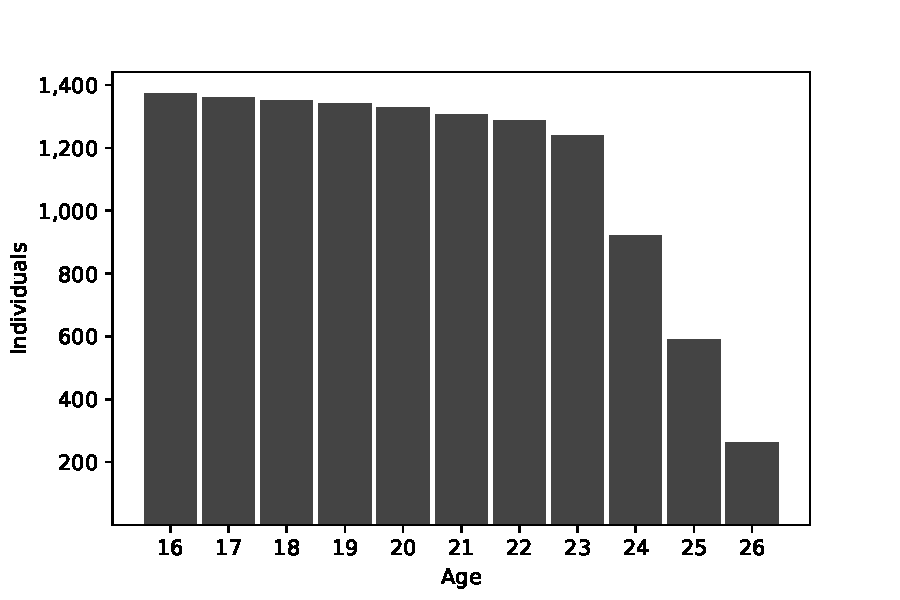
\includegraphics[scale=0.6]{fig-sample-size-bw}
\end{figure}

%-------------------------------------------------------------------------------
\subsection{Basic structure}
%-------------------------------------------------------------------------------
First we explore the basic structure of the dataset. All individuals enter the model initially at the same age and are then observed for a varying number of consecutive years. Each year, the individual’s decision to work in either a white or blue collar occupation, attend school, enroll in the military, or remain at home is recorded. If working, the dataset potentially also contains that year’s wage as a full-time equivalent. We show the data structure for an exemplary individual in Table \ref{tab:BasicDataStructure}.
\begin{ThreePartTable}
	% Information available at https://ftp.agdsn.de/pub/mirrors/latex/dante/macros/latex/contrib/threeparttablex/threeparttablex.pdf

	\begin{longtable}{@{}lccccccc@{}}
		\caption{Overview of the dataset structure from \citet{Keane.1997}.}
		\label{tab:BasicDataStructure}
		
		\setlength\extrarowheight{2.5pt}
		
		% Settings longtable
		\\
		\toprule
       & \textbf{Age}    & \thead{\textbf{Experience}\\ \textbf{Schooling}}  & \textbf{Choice} & \textbf{Wage} & \thead{\textbf{Experience}\\ \textbf{Blue Collar}} & \thead{\textbf{Experience}\\ \textbf{Blue Collar}} & \thead{\textbf{Experience}\\ \textbf{Military}}   \\
\textbf{Period} &        &            &        &      &             &               &       \\ \midrule
		\endfirsthead
		
		% Start table
0  & 16 & 11 & schooling    & - & - & - & -\\
1  & 17 & 12 & schooling    & - & 0 & 0 & 0\\
2  & 18 & 13 & schooling    & - & 0 & 0 & 0\\
3  & 19 & 14 & schooling    & - & 0 & 0 & 0\\
4  & 20 & 15 & schooling    & - & 0 & 0 & 0\\
5  & 21 & 16 & home         & - & 0 & 0 & 0\\
6  & 22 & 16 & white collar & 14,062.7 & 0 & 0 & 0\\
7  & 23 & 16 & white collar & 15,921.2 & 0 & 1 & 0\\
8  & 24 & 16 & white collar & 18,602.7 & 0 & 2 & 0\\
9  & 25 & 16 & white collar & 19,694.0 & 0 & 3 & 0\\
10 & 26 & 16 & white collar & 20,611.0 & 0 & 4 & 0\\
  \bottomrule
	\begin{TableNotes}
		\item \textbf{Note:} The listed individual is represented as an example. 
	\end{TableNotes}		
	\end{longtable}
\end{ThreePartTable}


%-------------------------------------------------------------------------------
\subsection{Basic descriptives}
%-------------------------------------------------------------------------------
We are able to reproduce the descriptive statistics from \citet{Keane.1997} and present some of them below. 

\subsubsection*{Choices}
Table \ref{tab:TotalChoices} depicts the total and Table \ref{tab:RelativeChoices} the relative choice frequencies of the individuals clustered by age. %Figure \ref{fig:RelativeChoices} shows a more visually appealing version of the relative choice frequencies. 

\begin{ThreePartTable}
	% Information available at https://ftp.agdsn.de/pub/mirrors/latex/dante/macros/latex/contrib/threeparttablex/threeparttablex.pdf

	\begin{longtable}[c]{@{}lrrrrrr@{}}
		\caption{Absolut choice frequencies.}
		\label{tab:TotalChoices}

		\setlength\extrarowheight{2.5pt}
		
		% Settings longtable
		\\
		\toprule
       & \thead{\textbf{Blue} \\ \textbf{Collar}}    & \thead{\textbf{White} \\ \textbf{Collar}}  & \textbf{Military} & \textbf{Schooling} & \textbf{Home} & \textbf{All}   \\
\textbf{Age} &        &            &        &      &         \\ \midrule
		\endfirsthead
		
		% Start table
16&	45 & 4    &	1	& 1178 &	145& 	1373 \\
17&	113&	 15   &	20	& 1014 &	197	 & 1359 \\
18&	331&	 92   & 70  & 561   &296 	& 1350 \\
19&	406&	 115	  & 107 & 420	&293	 & 1341 \\
20&	454&	 149	  & 113 & 341	&273	 & 1330 \\
21&	498&	 170	  & 106 & 275	&257	 & 1306 \\
22&	559&	 256	  & 90	& 169	 &212	 & 1286 \\
23&	546&	 336	  & 68	& 105	 &185 & 1240 \\
24&	416&	 284	  & 44	& 65	  &112	& 921 \\
25&	267&	 215	  & 24	& 24   &	61   &	591 \\
26&	127&  88  & 2   & 13  &	32   &	262 \\
\textbf{All} &	3762& 1724&	645 & 4165	& 2063 &	12359 \\

  \bottomrule
	\end{longtable}
\end{ThreePartTable}
\begin{ThreePartTable}
	% Information available at https://ftp.agdsn.de/pub/mirrors/latex/dante/macros/latex/contrib/threeparttablex/threeparttablex.pdf

	\begin{longtable}[c]{@{}lrrrrrr@{}}
		\caption{Relative choice frequencies.}
		\label{tab:RelativeChoices}

		\setlength\extrarowheight{2.5pt}
		
		% Settings longtable
		\\
		\toprule
       & \thead{\textbf{Blue} \\ \textbf{Collar}}    & \thead{\textbf{White} \\ \textbf{Collar}}  & \textbf{Military} & \textbf{Schooling} & \textbf{Home}   \\
\textbf{Age} &        &            &        &      &       \\ \midrule
		\endfirsthead
		
		% Start table
16&	3.28& 	0.29& 	0.07 &	85.80 &	 10.56 \\
17&	8.31	& 1.10&	1.47	 &74.61&	14.50 \\
18&	24.52&	6.81& 	5.19 &	41.56 &	21.93\\
19&	30.28&	8.58	& 7.98&	31.32 &	21.85\\
20&	34.14&	11.20 & 8.50&	25.64&	20.53\\
21&	38.13&	13.02&	8.12& 	21.06 &	19.68 \\
22&	43.47&	19.91&	7.00 &	13.14	&16.49\\
23&	44.03&	27.10& 	5.48	 &8.47&	14.92\\
24&	45.17&	30.84&	4.78	 &7.06 &	12.16\\
25&	45.18&	36.38&	4.06	& 4.06	& 10.32\\
26&	48.47&	33.59&	0.76&	 4.96&	12.21\\
\textbf{All}&	30.44&	13.95&	5.22	& 33.7 &	16.69\\


  \bottomrule
	\end{longtable}
\end{ThreePartTable}
%\begin{figure}[h]\centering
%\caption{Sample size with respect to the age.}\label{fig:RelativeChoices}
%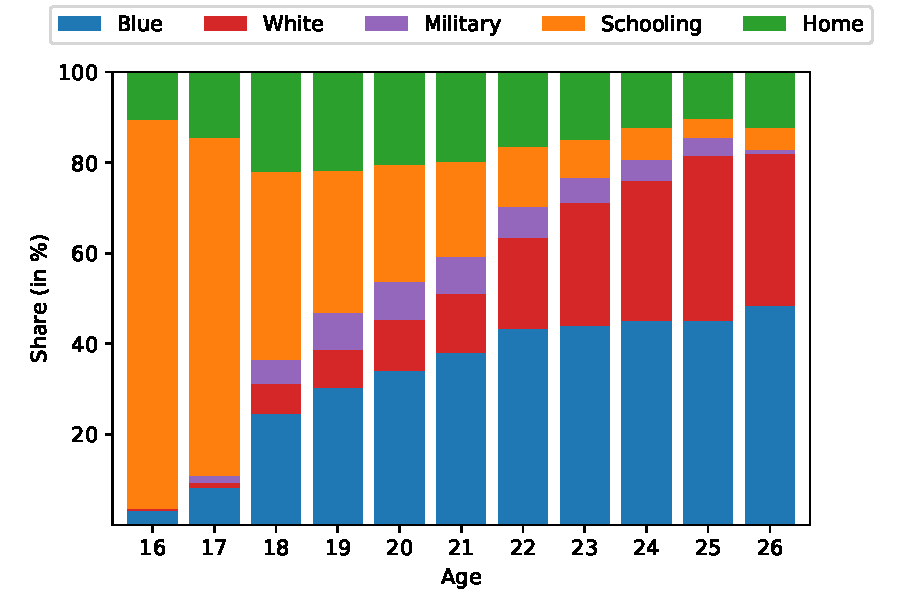
\includegraphics[scale=0.6]{fig-observed-data_choices}
%\end{figure}
Initially, roughly $86\%$ of the individuals are enrolled in school, but this share steadily declines with age. Nevertheless, about $39\%$ obtain more than a high school degree and continue their education for more than twelve years. As individuals leave school, most of them initially pursue a blue-collar occupation. But the relative share of the white-collar occupation increases as individuals entering the labor market later have higher levels of schooling. At age 26, about $48\%$ work in a white-collar occupation and $34\%$ in a blue-collar occupation. The share of individuals in the military peaks around age 20 with $8\%$. At its maximum around age 18, approximately $20\%$ of individuals stay at home.

\subsubsection*{Wages}
We reproduce the average real wages by occupation in Table \ref{tab:AverageWages} and plot the standard deviation by age in Figure \ref{fig:WageMoments}.

The average wages in the blue-collar occupation are initially highest with about \$10,286, while wages in the white-collar occupation and military start around \$9,000. However, wages in the white-collar occupation increase steeper over time and overtake blue-collar wages around age 21. At the end of the observation period, wages in the white-collar occupation are about $50\%$ higher compared to blue-collar wages with \$32,756 as opposed to only \$20,739. Military wages remain lowest throughout.
\newpage
\begin{ThreePartTable}
	% Information available at https://ftp.agdsn.de/pub/mirrors/latex/dante/macros/latex/contrib/threeparttablex/threeparttablex.pdf

	\begin{longtable}[c]{@{}lrrrr@{}}
		\caption{Average real wages by occupation.}
		\label{tab:AverageWages}

		\setlength\extrarowheight{2.5pt}
		
		% Settings longtable
		\\
		\toprule
       & \thead{\textbf{Blue-} \\ \textbf{Collar}}    & \thead{\textbf{White-} \\ \textbf{Collar}}  & \textbf{Military}  & \textbf{All}   \\
\textbf{Age} &        &         &  &       \\ \midrule
		\endfirsthead
		
		% Start table
16	&	10,286.74	&	9,320.76	&		- &	10,217.74 \\
17	&	11,572.89	&	10,049.76	&	9,005.36	&	11,036.60\\
18	&	12,603.82	&	11,775.34	&	10,171.87	&	12,060.75\\
19	&	12,949.84	&	12,376.42	&	9,714.60	&	12,246.68\\
20	&	14,363.66	&	13,824.01	&	10,852.51	&	13,635.87\\
21	&	15,313.45	&	15,578.14	&	12,619.37	&	14,977.00\\
22	&	16,947.90	&	20,236.08	&	13,771.56	&	17,561.28\\
23	&	17,884.95	&	20,745.56	&	14,868.65	&	18,719.84\\
24	&	19,245.19	&	24,066.64	&	15,910.84	&	20,942.42\\
25	&	21,473.31	&	24,899.23	&	17,134.46	&	22,754.54\\
26	&	20,738.91	&	32,756.04	&	25,216.83	&	25,390.90\\
All	&	16,436.96	&	20,295.00	&	12,255.75	&	17,115.60\\



  \bottomrule
	\end{longtable}
\end{ThreePartTable}

%\begin{figure}[h]\centering
%	\caption{Wage moments by age.}\label{fig:WageMoments}
%	\subfloat[White-collar]{\scalebox{0.38}{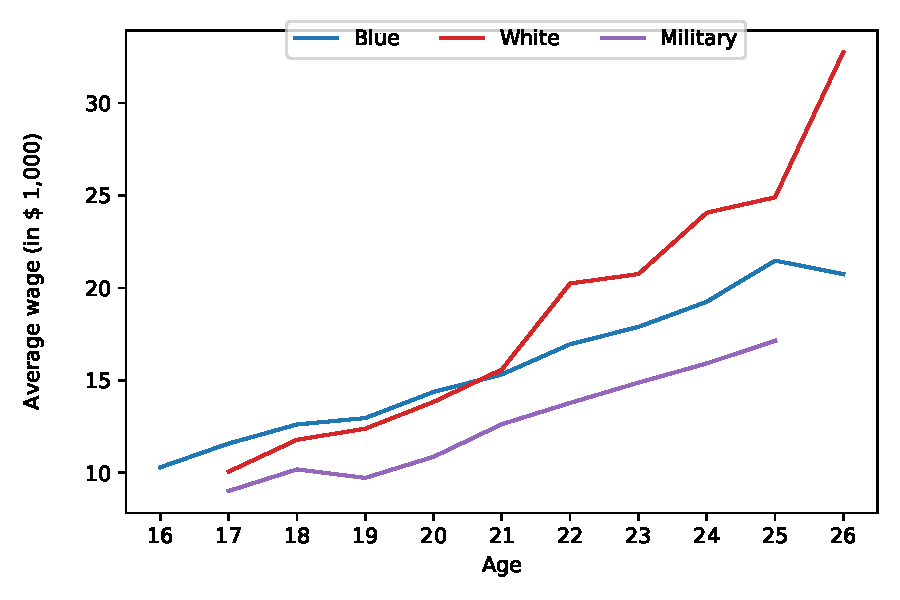
\includegraphics{fig-observed-wage-mean}}}\hspace{0.3cm}
%	\subfloat[Military]{\scalebox{0.38}{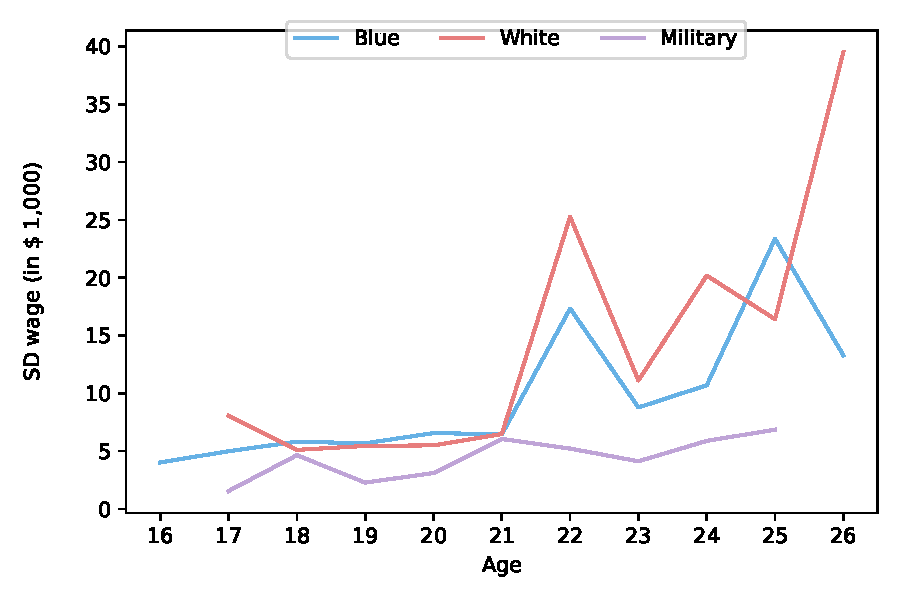
\includegraphics{fig-observed-wage-std}}} 
%	\floatfoot{\footnotesize \textbf{Note}: In the calculation of wage moments we have excluded data points (age) for which only less than 10 observations were available.}\\
%\end{figure}
\begin{figure}[h]\centering
\caption{Wage standard deviation by age.}\label{fig:WageMoments}
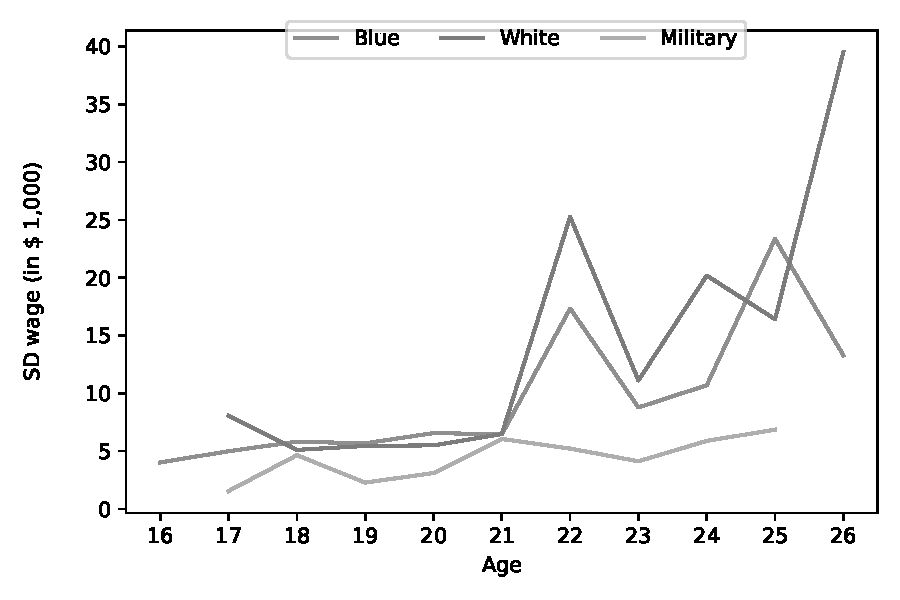
\includegraphics[scale=0.6]{fig-observed-wage-std-bw}
\floatfoot{\footnotesize \textbf{Note}: In the calculation of wage moments we have excluded data points (age) for which only less than 10 observations were available.}
\end{figure}

\subsubsection*{Initial schooling}

Individuals that enter the model differ with respect to their unobservable type $\{e_{a,t}\}_{a \in \mathcal{A}}$ and the level of initial schooling. The following table and figure illustrate the distribution of initial schooling. Two-thirds of individuals ($67.15\%$) enter with 10 years of schooling, while $20.18 + 4.22 + 0.01 = 24.41\%$ of individuals have less than 10 years of schooling, and $7.5\%$ of individuals were 11 years in school. The average years of initial schooling in the sample amounts to 9.76 years.
\begin{ThreePartTable}
	% Information available at https://ftp.agdsn.de/pub/mirrors/latex/dante/macros/latex/contrib/threeparttablex/threeparttablex.pdf

	\begin{longtable}[c]{@{}lrr@{}}
		\caption{Initial years of schooling.}
		\label{tab:InitialSchooling}

		\setlength\extrarowheight{2.5pt}
		
		% Settings longtable
		\\
		\toprule
\textbf{Years} & \textbf{Number} & \textbf{Frequency} \\ \midrule
		\endfirsthead
7 & 13 & 0.01 \\
 8 & 58 & 0.04 \\
 9 & 277 & 0.20 \\
10 & 922 & 0.67 \\
11 & 103 & 0.08\\	

  \bottomrule
	\end{longtable}
\end{ThreePartTable}
\begin{figure}[h]\centering
\caption{Distribution of initial schooling.}\label{fig:InitialSchooling}
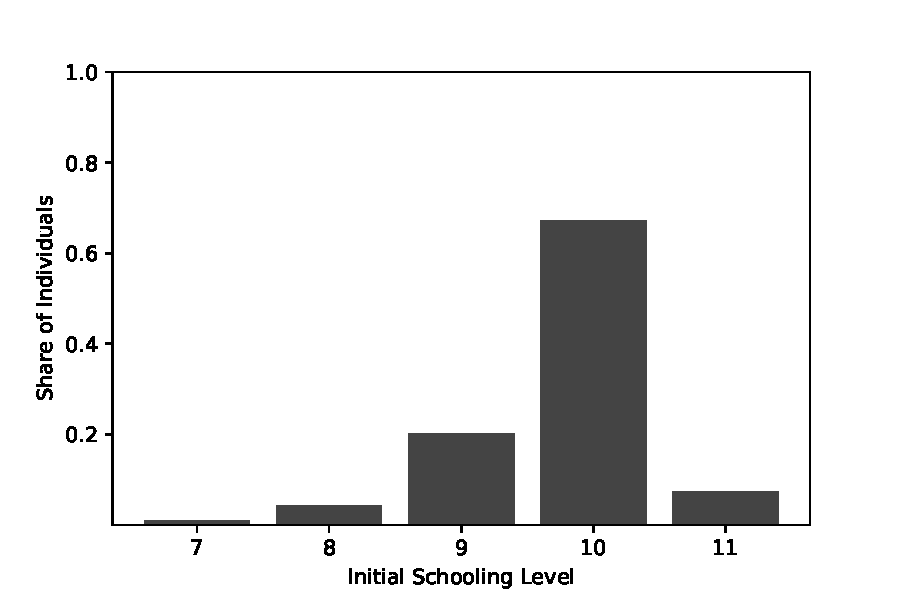
\includegraphics[scale=0.6]{fig-initial-schooling-bw}
\end{figure}

The amount of schooling an individual obtains is an important determinant for life cycle decisions. The following table illustrates the years spent on each activity by the initial level of schooling.
\begin{ThreePartTable}
	% Information available at https://ftp.agdsn.de/pub/mirrors/latex/dante/macros/latex/contrib/threeparttablex/threeparttablex.pdf

	\begin{longtable}[c]{@{}lrrrrr@{}}
		\caption{Average choice frequencies with respect to the initial years of schooling.}
		\label{tab:InitialSchoolingActivity}

		\setlength\extrarowheight{2.5pt}
		
		% Settings longtable
		\\
		\toprule
		
		% Start table
   &	\textbf{7}	&	\textbf{8}	&	\textbf{9}	&	\textbf{10}	&	\textbf{11}	\\ \midrule
		\endfirsthead
\textbf{Blue-Collar}	&	4.15	&	4.18	&	4.06	&	3.15	&	3.19	\\
\textbf{White-Collar}	&	0.10	&	0.27	&	0.54	&	1.03	&	1.21	\\
\textbf{Military}&	0.02	&	0.11	&	0.35	&	0.51	&	0.68	\\
\textbf{School}	&	0.12	&	0.29	&	1.00	&	2.35	&	2.56	\\
\textbf{Home}	&	5.00	&	4.50	&	3.21	&	2.11	&	1.58	\\
\textbf{Total}	&	9.39	&	9.36	&	9.17	&	9.16	&	9.23	\\



  \bottomrule
	\end{longtable}
\end{ThreePartTable}

Years spent in blue-collar occupations decrease with the initial level of schooling. While individuals with 7 years of initial schooling work on average 4.15 in a blue-collar occupation, individuals that have 11 years of schooling spend only 3.19 years in a blue-collar occupation. Years spent in white-collar occupations increase with the initial level of schooling. In particular, nearly no individual with only 7 years of schooling is occupied in a white-collar job. While individuals at the top distribution spend on average 1.21 years in white-collar ocucpations. The initial level of schooling is a strong predictor for additional schooling. While individuals who enter the model with only 7 years of schooling do not even spend 2 more month in school (on average), those with 11 years of initial schooling add on average 2.5 years. Notably, the descriptives are derived under the instance that the average duration of individuals in the sample differs by the level of initial schooling. Individuals with 7 years of initial schooling are observed for 9.4 periods, while individuals with 10 years of initial schooling are only observed for 9.16 years.

\subsubsection*{Transition matrix}
We illustrate two directions of transition probabilities. Table \ref{tab:TransitionProbabilitiesOriginToDestination} depicts the transition probabilities from the choice origin to the choice destination, this is to say, the percentage of individuals who are in an originating alternative in period $t$ (column) and will be in a destination alternative in period $t+1$ (row).
\begin{ThreePartTable}
	% Information available at https://ftp.agdsn.de/pub/mirrors/latex/dante/macros/latex/contrib/threeparttablex/threeparttablex.pdf

	\begin{longtable}[c]{@{}lrrrrrr@{}}
		\caption{Transition probabilities from origin to destination.}
		\label{tab:TransitionProbabilitiesOriginToDestination}

		\setlength\extrarowheight{2.5pt}
		
		% Settings longtable
		\\
		\toprule
   & \thead{\textbf{Blue-} \\ \textbf{Collar}}    & \thead{\textbf{White-} \\ \textbf{Collar}}  & \textbf{Military} & \textbf{Schooling} & \textbf{Home}   \\ \midrule
		\endfirsthead
		
		% Start table
\textbf{Blue-Collar}	&	0.73	&	0.10	&	0.01	&	0.03	&	0.12	\\
\textbf{White-Collar	} &	0.20	&	0.67	&	0.01	&	0.06	&	0.06	\\
\textbf{Military	} &	0.10	&	0.03	&	0.80	&	0.01	&	0.06	\\
\textbf{Schooling}	&	0.12	&	0.09	&	0.02	&	0.64	&	0.13	\\
\textbf{Home	} &	0.31	&	0.08	&	0.04	&	0.10	&	0.47	\\
  \bottomrule
	\end{longtable}
\end{ThreePartTable}
Table \ref{tab:TransitionProbabilitiesDestinationToOrigin} depicts the transition probabilities from the choice destination to the choice origin, this is to say, the percentage of individuals who are in a destinating alternative in period $t$ (column) and were in a certain originating alternative in period $t-1$ (row).
\begin{ThreePartTable}
	% Information available at https://ftp.agdsn.de/pub/mirrors/latex/dante/macros/latex/contrib/threeparttablex/threeparttablex.pdf

	\begin{longtable}[c]{@{}lrrrrrr@{}}
		\caption{Transition probabilities from destination to origin.}
		\label{tab:TransitionProbabilitiesDestinationToOrigin}

		\setlength\extrarowheight{2.5pt}
		
		% Settings longtable
		\\
		\toprule
   & \thead{\textbf{Blue-} \\ \textbf{Collar}}    & \thead{\textbf{White-} \\ \textbf{Collar}}  & \textbf{Military} & \textbf{Schooling} & \textbf{Home}   \\ \midrule
		\endfirsthead
		
		% Start table
\textbf{Blue	-Collar }&	0.62	&	0.07	&	0.02	&	0.13	&	0.16	\\
\textbf{White-Collar	}&	0.18	&	0.52	&	0.01	&	0.20	&	0.09	\\
\textbf{Military}	&	0.04	&	0.01	&	0.73	&	0.11	&	0.11	\\
\textbf{Schooling}	&	0.04	&	0.03	&	0.00	&	0.87	&	0.06	\\
\textbf{Home}	&	0.20	&	0.04	&	0.02	&	0.27	&	0.46	\\
  \bottomrule
	\end{longtable}
\end{ThreePartTable}

The diagonal indicates that choices are quite persistent. There is limited mobility between white and blue collar occupations. However, more people transition from a white-collar to a blue-collar occupation than from a white-collar to a blue-collar occupation. Blue-collar workers are twice more likely to transition into home than white-collar workers. Individuals who are not in school at a certain will most likely not return to school.


In the original data set choices at age 15 are not available. Consequently, the transition probabilities reported in Table 2 from \citet{Keane.1997} cannot be replicated. However, their transition probabilities can be approximated by imputing schooling exprience for individuals at age 15. We use the following rule: If an individual at age 16 has 9 or more years of schooling, then he was in school at age 15. If an individual at age 16 has less than 9 years of schooling, then he was not in school at age 15. The new transition probabilities for schooling are closer to those reported in \citet{Keane.1997}.
\begin{ThreePartTable}
	% Information available at https://ftp.agdsn.de/pub/mirrors/latex/dante/macros/latex/contrib/threeparttablex/threeparttablex.pdf

	\begin{longtable}[c]{@{}lrrrrrr@{}}
		\caption{Transition probabilities from origin to destination with imputed schooling exprience for individuals at age 15.}
		\label{tab:TransitionProbabilitiesImputing}

		\setlength\extrarowheight{2.5pt}
		
		% Settings longtable
		\\
		\toprule
   & \thead{\textbf{Blue-} \\ \textbf{Collar}}    & \thead{\textbf{White-} \\ \textbf{Collar}}  & \textbf{Military} & \textbf{Schooling} & \textbf{Home}   \\ \midrule
		\endfirsthead
		
		% Start table
\textbf{Blue-Collar}	&	0.73	&	0.10	&	0.01	&	0.03	&	0.12	\\
\textbf{White-Collar	} &	0.20	&	0.67	&	0.01	&	0.06	&	0.06	\\
\textbf{Military	} &	0.10	&	0.03	&	0.80	&	0.01	&	0.06	\\
\textbf{Schooling}	&	0.10&	0.07	&	0.01	&	0.70	&	0.12	\\
\textbf{Home	} &	0.31	&	0.08	&	0.04	&	0.10	&	0.47	\\
  \bottomrule
	\end{longtable}
\end{ThreePartTable}


\newpage
\subsection{Model fit}

We provide a full stack of comparisons between simulated and empirical data. We simulate a sample of 1,000 individuals using the calibrated model.



\begin{figure}[h]\centering
	\caption{Model fit}\label{Model fit appendix}
	\subfloat[White-collar]{\scalebox{0.19}{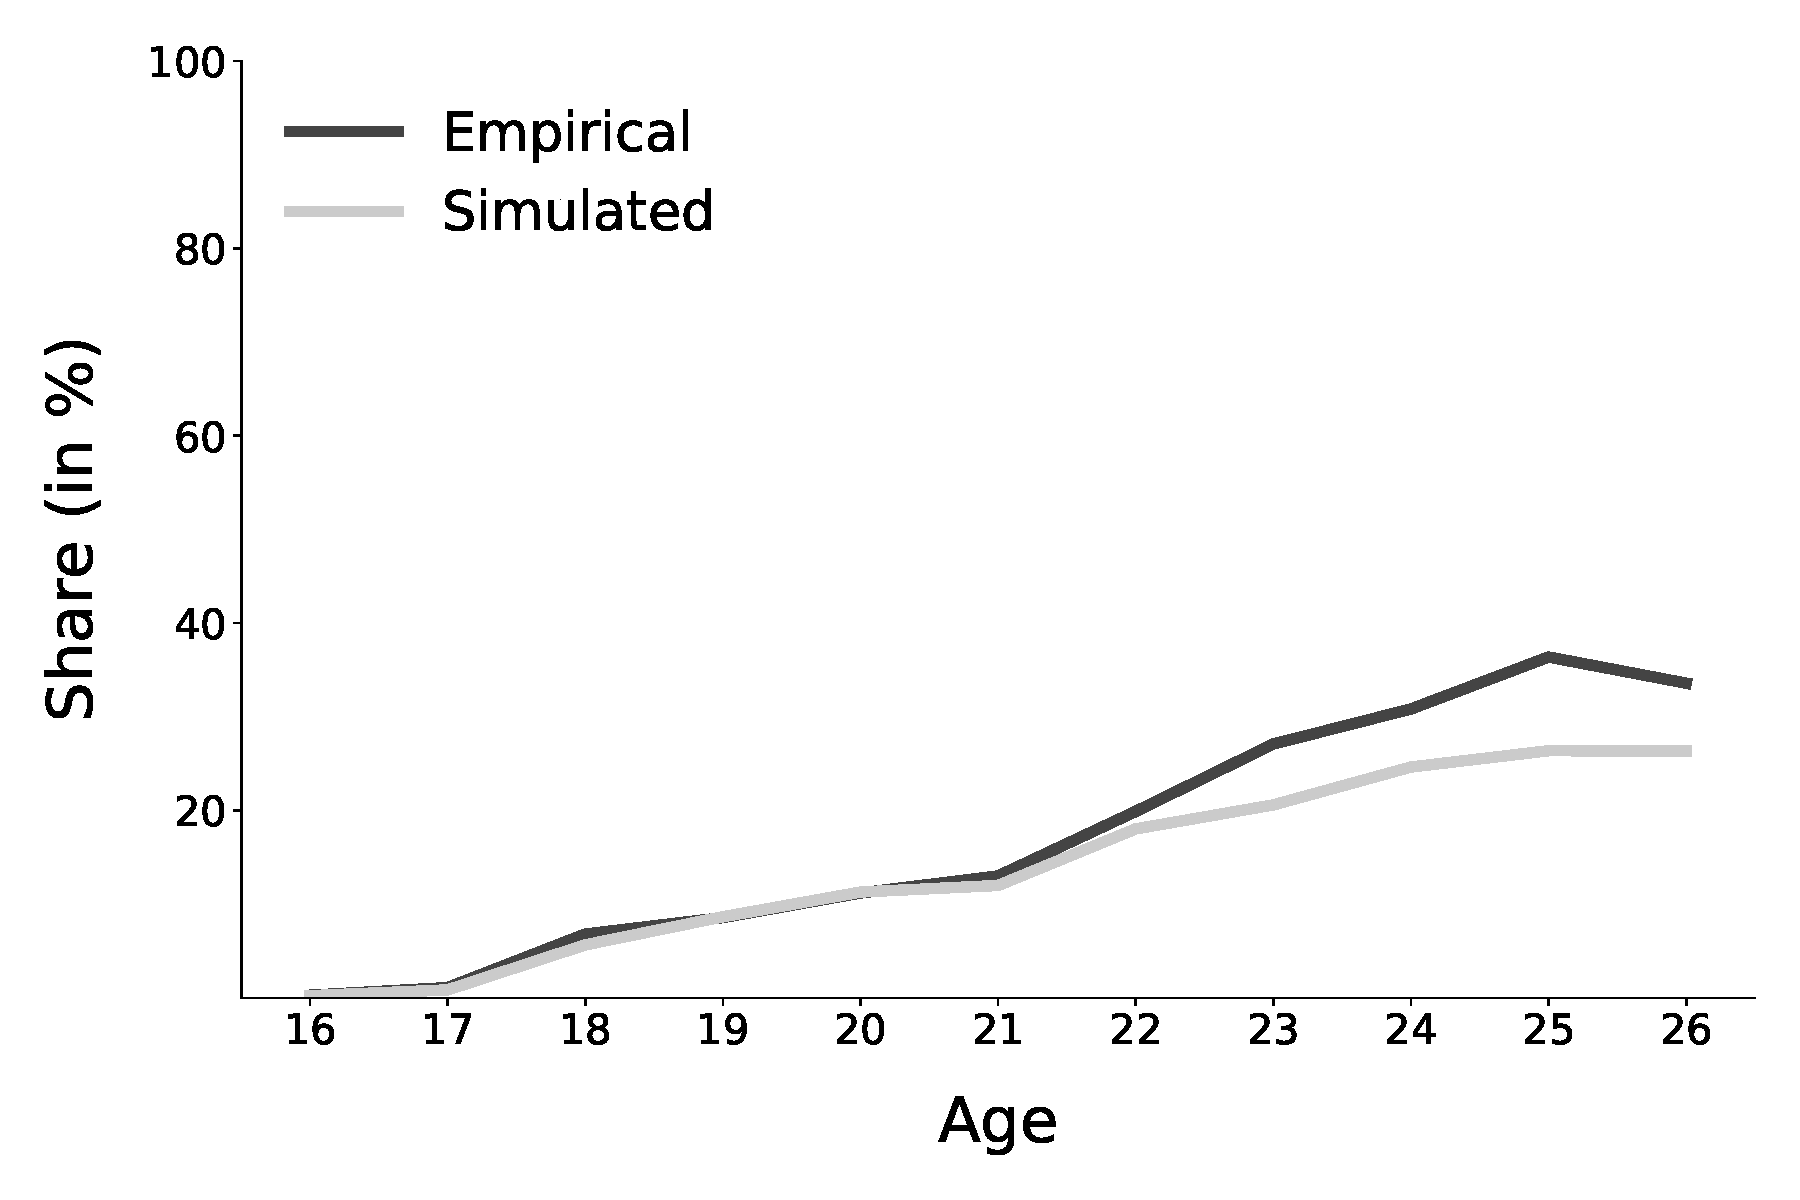
\includegraphics{fig-model-fit-choice-white-bw}}}\hspace{0.3cm}
	\subfloat[Military]{\scalebox{0.19}{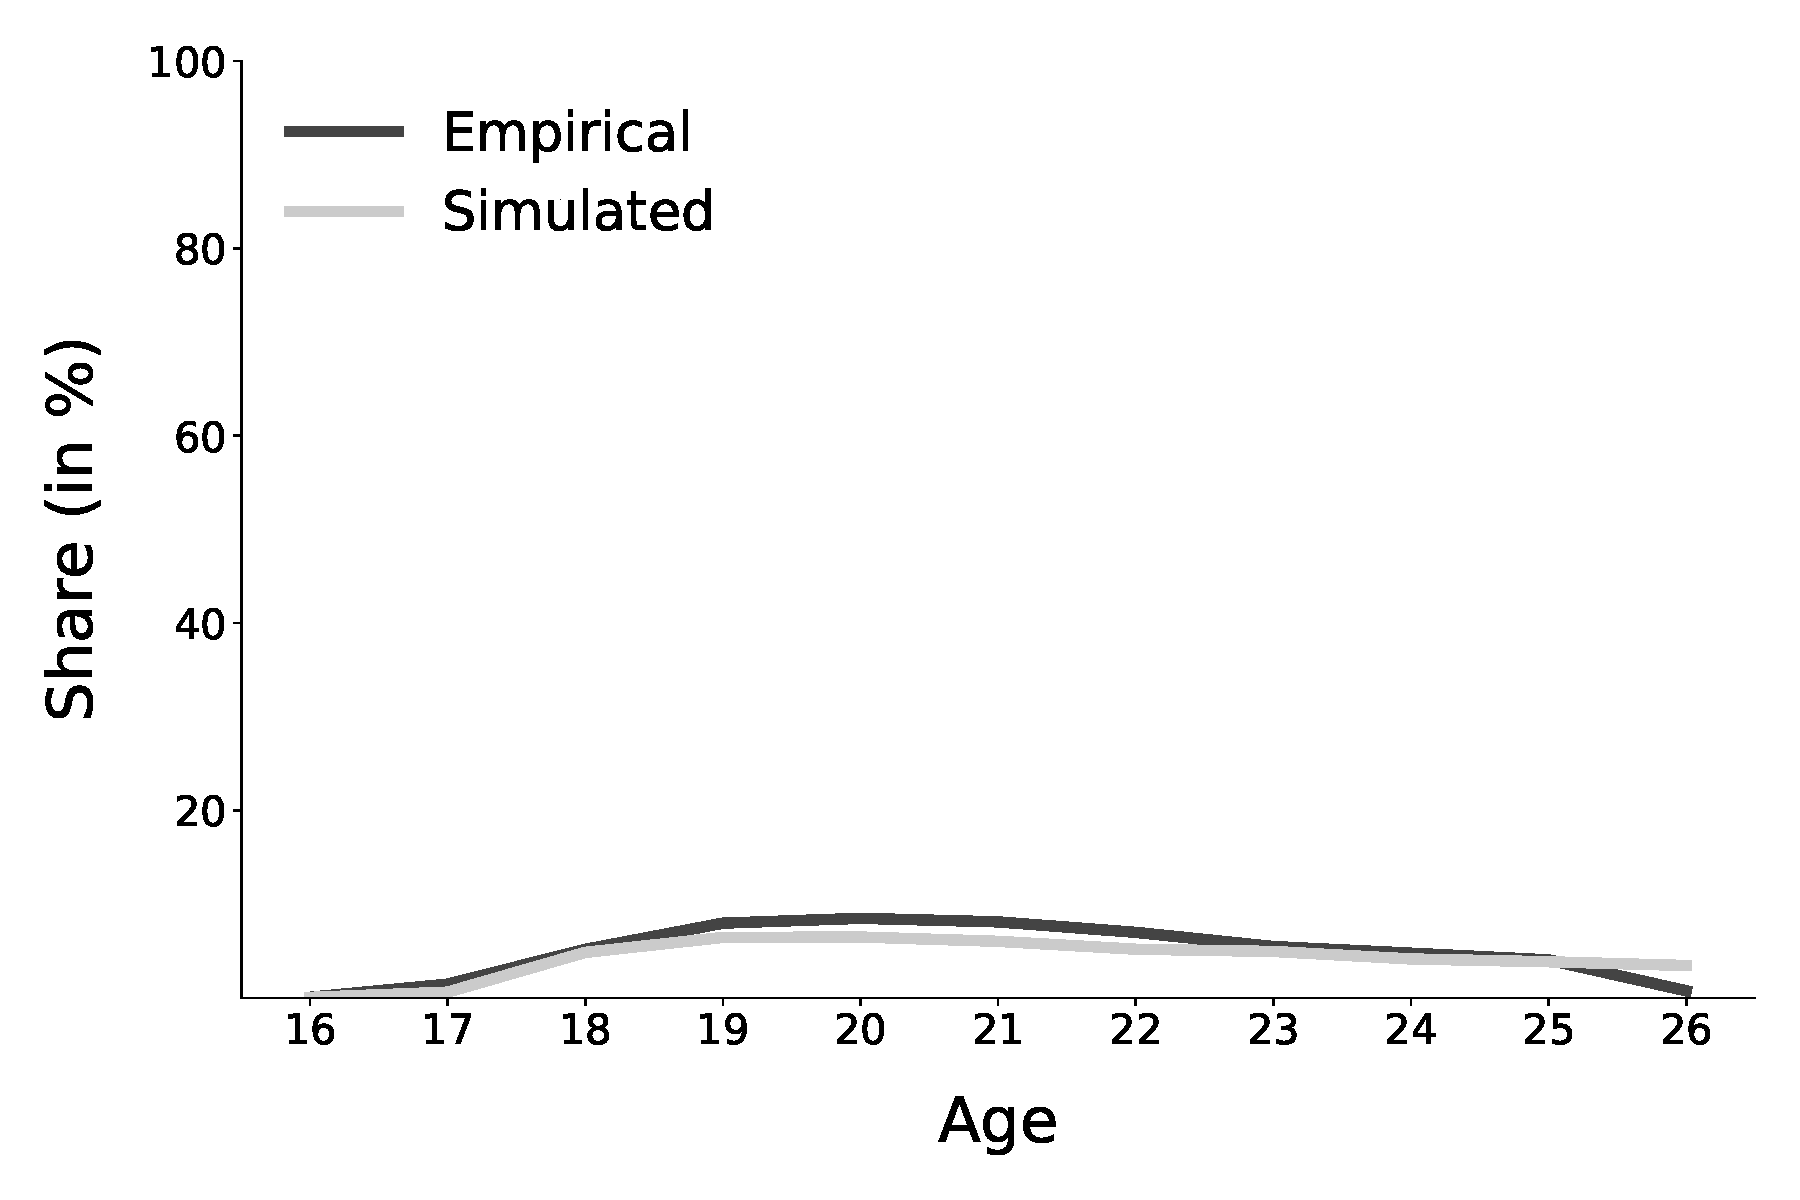
\includegraphics{fig-model-fit-choice-military-bw}}} \\
	\subfloat[School]{\scalebox{0.19}{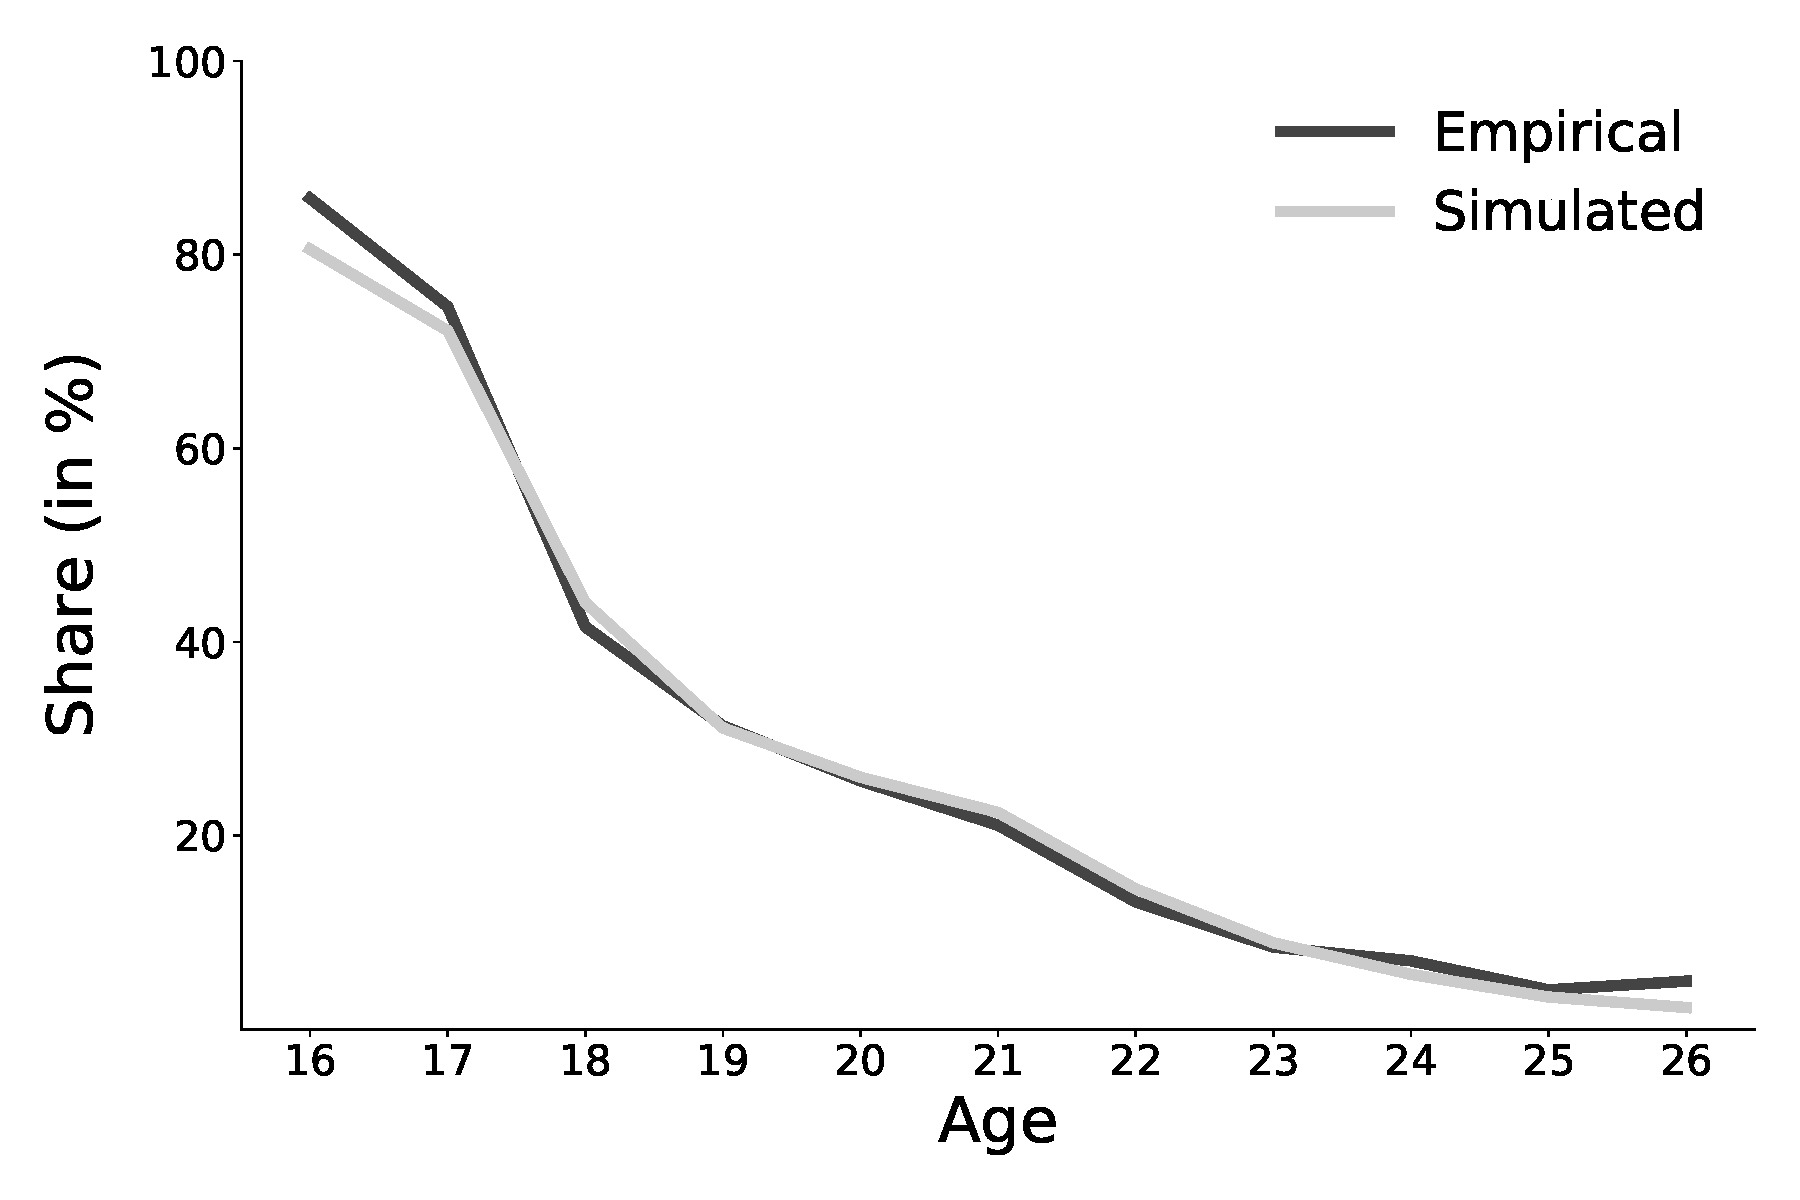
\includegraphics{fig-model-fit-choice-school-bw}}}\hspace{0.3cm}
	\subfloat[Home]{\scalebox{0.19}{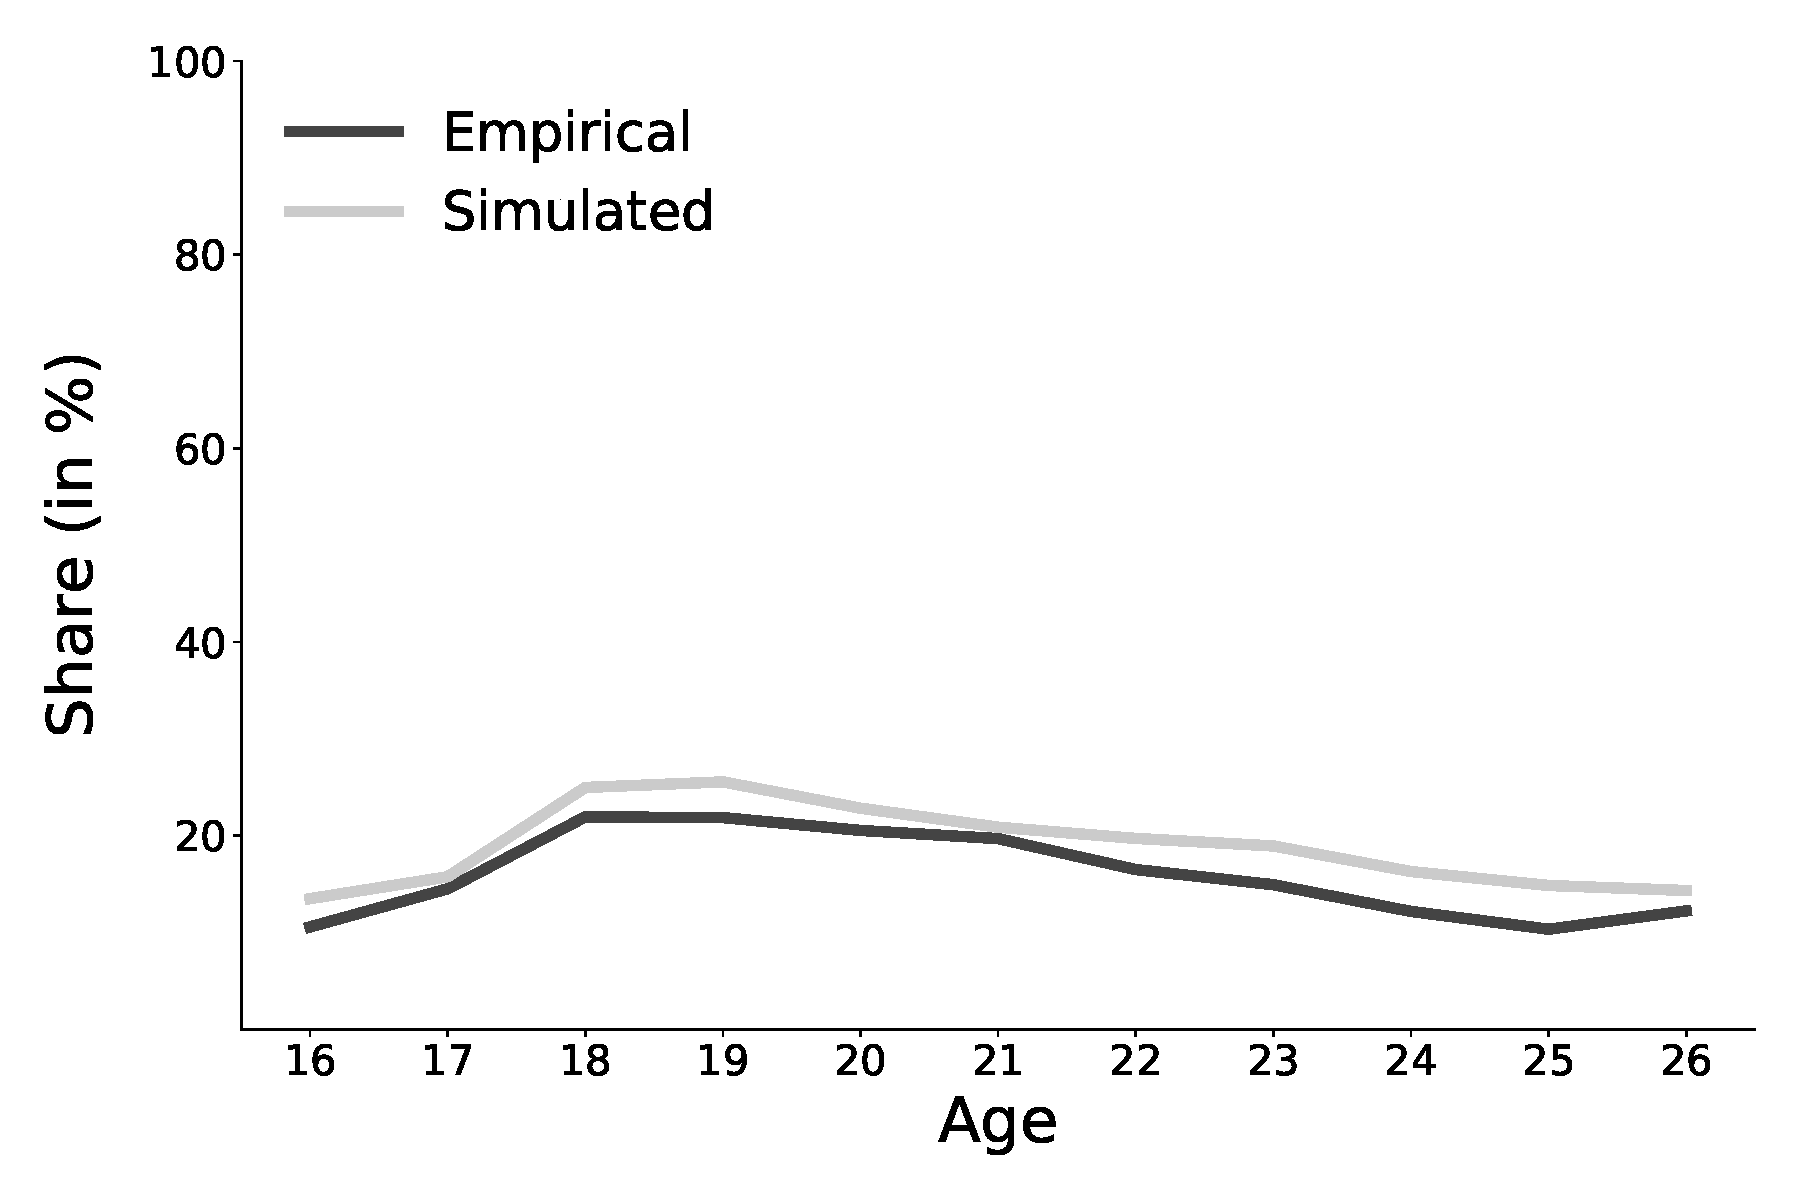
\includegraphics{fig-model-fit-choice-home-bw}}}
\end{figure}


